\subsection{The oblate spheroidal fluid particles}


% \subsubsection{Shape description of the droplet}
As discussed in \ref{sec:intro_ellipse} we consider that all particles posses an oblate spheroidal shape as represented \ref{fig:scheme_spheroid}. 
This shape is advantageous, since for small deformation, it is shown based on theoretical ground that droplets and bubble adopt an ellipsoidal shape, either for particle in relative translation \citep{taylor1964deformation} or immersed in a pure linear flows \citet{leal2007advanced}. 
However, it is true that a droplet immersed in quadratic flows does not deform as an ellipsoid, see \citep{nadim1991motion}, meaning that for instance we must neglect the quadratic contribution for the carrier fluid in the closure problem. 
\begin{figure}[h!]
    \centering
    \hfill
    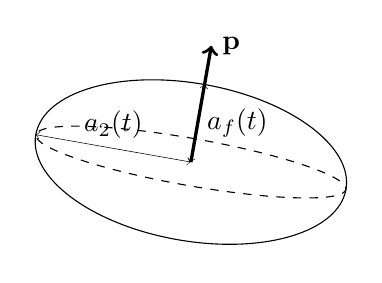
\begin{tikzpicture}[rotate=80]
        \draw(0,0) ellipse (1 cm and 2 cm);
        \draw[dashed](0,0) ellipse (0.3 cm and 2 cm);
        \draw[<->,very thin](0,0) --++ (1,0)node[midway,right]{$a_f(t)$};
        \draw[->,very thick](0,0) --++ (1.5,0)node[right]{$\textbf{p}$};
        \draw[<->,very thin](0,0) --++ (0,2)node[midway,above]{$a_2(t)$};
    \end{tikzpicture}
    \hfill
    \caption{Scheme of an  oblate spheroid oriented along the unit vector \textbf{p} with $a_f(t)$ and $a_2(t)$ the length of the semi axes of the spheroid.
    Note that when the drop is spherical we have $a_f=a_2=a$}
    \label{fig:scheme_spheroid}
\end{figure}

The shape of the particle is entirely described by an orientation vector $\textbf{p}$ and its two semi axis, $a_1$ and $a_2$.  
By direct integration over the spheroidal particle volume in its local reference frame, one may directly find that $M_1$ and $M_2$ which are the eigenvalues of $\textbf{M}_\alpha$, read as 
\begin{align*}
    M_1 = \frac{m_\alpha a_1^2}{5}
    && M_2 = \frac{m_\alpha a_2^2}{5}
\end{align*}
Since the particle volume remains constant over time  \eqref{eq:dt_m_alpha}, we can state that $a_2^2 a_1 =a^3$, where $a$ is the radius of the equivalent spherical particle. 
We measure the deviation from the spherical shape with the dimensionless properties: $\chi_I = (a_1/a)^2 - 1$ and $\chi_{II} = (a_2/a)^2 - 1$. 
With this definition, $\chi_I = 0$ when, $a_1/a =1$ implying a spherical shape. 
$\chi_I$ will be termed the first aspect ratio of the droplet.  
Based on these definitions, the volume conservation \eqref{eq:dt_m_alpha} implies that $\chi_{II} = (\chi_I + 1)^{-1/2} - 1$.
% $a_2^2 a_1 =a^3 \to \chi_{II} + 1 = a /a_1$
% $\chi_I = (a_1/a)^2 - 1 \to (\chi_I +1)^{-1/2} = a/a_1$
% $a_1/a = a^2/a_2^2$
% Thus, the droplets shape is entirely determined by its orientation vector and one of its aspect ratio $\chi_I = a_1/a$ or $\chi_{II} = a_2^2/a^2$. 
Considering all these remarks we may describe the droplet shape using the dimensionless tensor, 
\begin{equation*}
    \bm\chi_\alpha
    = \frac{5}{m_\alpha a^2}(\textbf{M}_\alpha - \bm\delta)
    = \chi_I \textbf{pp}
        +[(\chi_I + 1)^{-1/2} - 1 ] (\bm\delta - \textbf{pp}). 
\end{equation*}
Thus, the droplet spheroidal shape, is entirely characterized by two relevant parameters: the orientation vector \textbf{p} and its aspect ratio $\chi_I$.
It is interesting to notice that since $\textbf{p}$ is an eigenvector of $\textbf{M}_\alpha$ and $\bm\chi_\alpha$, $\chi_I$ and $\chi_{II}$ constitute the eigenvalues of $\bm\chi_\alpha$. 
Notice that with the definition used here, $\bm\chi_\alpha +\bm\delta$ correspond to the Cauchy green deformation tensor often employed in solid mechanics \citep{mwasame2018macroscopic}. 
The geometrical description of the surface of the droplet can also be obtained using the tensor $\bm\chi_\alpha$. 
Indeed, we introduce the distance function  $\FF_\alpha$, describing the ellipsoidal surface of the particle as \citep{nadim1996concise},  
\begin{equation*}
    \FF_\alpha(\textbf{x}_\alpha +\textbf{r},t) = \textbf{rr}:(\bm\chi_\alpha +\bm\delta)-a^2.  
    \label{eq:distance_function}
\end{equation*}
It is to be understood from this definition that the points $\textbf{x}$ lying on the surface of the particles respect the constraint $\FF_\alpha(\textbf{x},t) = 0$. 
Being able to define the droplet's surface in this way will find its use in the calculation of the surface tension stress term present in \ref{eq:dt_S_alpha}. 

% \begin{remark}{Hypothesis of small deformation :}
    
% \end{remark}
\paragraph*{Hypothesis of small deformation: }
A droplet in a pure linear flow will deform into an ellipsoidal shape \citet{leal2007advanced}. 
A buoyant rising droplet with the effect of small inertia will deform at the first order in $Re$ into an ellipsoid as well \citep{taylor1964deformation} .
However, as soon as the inertial effect may be higher or that the flow becomes no-more linear but quadratic for exemple, the droplets' deformation is found to exhibit other shapes than ellipsoid \citet{taylor1964deformation,stone1990simple}.
Therefore, in this work we limit our study to small deformations, since as soon as the droplet deformation reaches high value one might expect other shapes than ellipsoid, which is in contradiction with the initial assumption. 
Thus, in order to stay within our study's hypothesis we may consider only small deformation. 
This means that we neglect all the term of $\mathcal{O}(\chi_I^2)$ or $\mathcal{O}(\chi_{II}^2)$ or higher. 
In this situation notice that $\chi_{II} = (\chi_I + 1)^{-1/2} -1 \approx  - \chi_I /2$. 
Thus, the deformation tensor can be written in the simple form, 
\begin{equation*}
    \bm\chi 
    = \chi_I
    \left[
        \textbf{pp} 
        - \frac{1}{2}(\bm\delta - \textbf{pp})
    \right]
    = \chi_I \frac{1}{2} \left[
        3 \textbf{pp} - \bm\delta
    \right]
\end{equation*}
Thus, the trace of $\bm\chi_\alpha$ may be written for small deformation as :  $\frac{1}{3}\bm\delta:\bm\chi_\alpha  = \chi_I + 2\chi_{II} = \mathcal{O}(\chi_{I}^2)$. 
Notice that in the next order of deformation we have $\frac{1}{3}\bm\delta:\bm\chi_\alpha  = \chi_I + 2\chi_{II} = 3 \chi_I^2 /4 +  \mathcal{O}(\chi_{I}^3)$. 
In other worlds the trace of $\bm\chi_\alpha$ is null only when considering small deformation, this property will find its use in the following sections. 


\subsection{The droplet's internal velocity}

Now that the droplet shape is properly defined we turn our attention to the description of the internal flow present within the droplets.
Indeed, the droplets internal flow $\textbf{w}_d^0$ present in the closure term of \ref{eq:dt_S_alpha} is not part of the Lagrangian unknown, and therefore must be either directly closed or related to the Lagrangian properties which are the unknown of the problem.  
To simplify the conservation equations in \citet{lhuillier1987phenomenology} they simply assume that the flow within the droplets is linear with the position. 
In our notation it means that $\textbf{w}_d^0 = \textbf{r}\cdot \textbf{E}_\alpha(t)$ where $\textbf{E}_\alpha(t)$ corresponds to the mean rate of strain of the particle. 
In this case $\textbf{E}_\alpha(t)$ constitutes an unknown of the particle phase which is solved in \citet{lhuillier1987phenomenology} with an equation similar to \ref{eq:dt_S_alpha}. 
For deformable solid bodies this approach is accurate since the internal velocity field is indeed linear.
Nevertheless, as discussed in \citet{lhuillier1987phenomenology} for fluid droplets, the internal velocity field $\textbf{w}_d^0$ is far from being linear, as $\textbf{w}_d^0$ exhibits complicated fluid circulation in most of the situations, and this hypothesis is somewhat doubtful. 
Consequently, in this work, we adopt a more general approach that sill accounts for the internal flows of the particles while limiting the Lagrangian unknowns.

It is known that an isolated droplet in creeping flow with relative translating motion with the carrier fluid exhibit internal motions. In this specific situation the streamlines formed by $\textbf{w}_d^0$ are known as Hill vortexes, see \ref{fig:flowlines} (b). 
If slightly more inertial effects are present the initially spherical droplet deform into an oblate spheroid \citep{taylor1964deformation}, and one might find that the internal motion are close to hill's vortexes but with an overall oblate spheroidal shape, see \ref{fig:flowlines} (c). 
For a drop immersed in an unbounded linear flow, still in stokes flows, we can derive an analytical solution for $\textbf{w}_d^0$ and find that $\textbf{w}_d^0 \sim \textbf{rrr}$, see \ref{fig:flowlines} (a). 
Thus, in all those cases the internal motions are way more complicated than a simple linear velocity field. 
Moreover, in all of those cases the droplet's internal velocity fields is a steady solution.
However, for a droplet to go from the state represented \ref{fig:flowlines} (b) to case \ref{fig:flowlines} (c) the droplet must deform from a sphere to an oblate ellipsoid. 
Equally, a droplet in a shearing flow may experience deformation and in that case $\textbf{w}_d^0$ may be function of time \citet[chapter 7]{leal2007advanced}.
\begin{figure*}
    \centering
    \begin{tikzpicture}
        \node (img3) at (0.6\textwidth,0) {\includegraphics[width=0.3\textwidth,angle=270]{image/Rising_def_Stokes.png}};
        \node (img2) at (0.3\textwidth,0) {\includegraphics[width=0.3\textwidth]{image/Rising_Stokes.png}};
        % \draw (0.45\textwidth,0)node{$\rightarrow$};
        % \draw (0.45\textwidth,0.4cm)node{$\bm\Gamma_\alpha\cdot \textbf{r}$};
        \node (img1) at (0.0\textwidth,0) {\includegraphics[width=0.3\textwidth]{image/Shear_Stokes.png}};
        \draw (img3.south)node{(c)};
        \draw (img2.south)node{(b)};
        \draw (img1.south)node{(a)};
    \end{tikzpicture}
    \caption{Three examples of steady state flow lines plots of an isolated droplet immersed into a viscous fluid. 
    (a) Rising sphere in uniform stokes flow (analytical solution in \ref{ap:Translating_sphere}). 
    (b) Fixed droplet in extensional flow (analytical solution in \ref{ap:Translating_sphere}).
    (c) Deformed droplet in rising motion (analytical solution of \citet{taylor1964deformation}). }
    \label{fig:flowlines}
\end{figure*} 
To account for this deformation in our case we assume that the \textit{transient internal velocity field} which is responsible for this deformation is homogeneous and linear with position \textbf{r}. 
Thus, the \textit{transient internal velocity field} of a particle can be modeled as $\textbf{w}_d^0 = \bm\Gamma_\alpha \cdot \textbf{r}$, were we have introduced, $\bm\Gamma_\alpha$, the mean velocity gradient inside the particle, which symmetric part : $\textbf{E}_\alpha$, represents the rate of strain, and skew symmetric part : $\bm\Omega_\alpha$, represents the angular velocity. 
Note that the angular velocity tensor $\bm\Omega_\alpha$ is related to the angular velocity \textit{pseudo} vector with the relation $-\frac{1}{2}\epsilon_{ijk} (\textbf{E}_\alpha)_{jk}$. 

To summarize, we assume that the inner velocity field of the drop can be decomposed into two distinct part. 
The first one is the steady state component, examples are : hill's vortex for spherical drop in steady linear motion, the hill'vortexes-like velocity field observed for oblate spheroidal droplets in translation,  the inner velocity field of a drop in steady linear flows, and so on\ldots 
The second contribution is the inner velocity fields that alter the drop's shape, this field is assumed linear with the position and homogeneous, that is $\bm\Gamma_\alpha\cdot \textbf{r}$. 
Adopting these definitions, the particle internal velocity is decomposed as, 
\begin{equation}
    \textbf{w}_{d}^0(\textbf{x}_\alpha)
    = \bm\Gamma_{\alpha}(t) \cdot \textbf{r}
    + \textbf{v}^0_{i}(t,\textbf{r})
    =\bm{\Omega}_{\alpha}\cdot \textbf{r}
    + \textbf{E}_{\alpha} \cdot \textbf{r}
    + \textbf{v}^0_{d}(t,\textbf{r})
    \label{eq:def_vel}
\end{equation}
Where we introduced the vector $\textbf{v}^0_d(t,\textbf{r}) =\textbf{v}^{0}_{d}(t,\textbf{r})  - \bm\Gamma_{\alpha}(t) \cdot \textbf{r}$.
With this definition $\textbf{v}_d^0$ represents all the particles internal that does not contribute to the linear homogeneous deformation. 
For example, $\textbf{v}_d^0$ could be one of the three velocity field presented in \ref{fig:flowlines}. 

An important consequence of this definition is that the integral on the RHS of \ref{eq:dt_M_alpha} is null when $\bm\Gamma_\alpha = 0$, i.e. when the particle does not deform. 
This can be shown by rewriting the second moment of mass equation with the use of the velocity decomposition.
Indeed, substituting $\textbf{w}_d^0$ with \ref{eq:def_vel} in \ref{eq:dt_M_alpha} gives directly,
\begin{equation*}
    \ddt \textbf{M}_{\alpha,ik}
    = 
    \textbf{M}_{\alpha,ik} \cdot \bm\Gamma_{\alpha,kj}
    +  \bm\Gamma_{\alpha,ki} \cdot \textbf{M}_{\alpha,jk}
    +
    \intO{ 
        (\textbf{v}_{d,i}^0\textbf{r}_j
        + \textbf{r}_i\textbf{v}_{d,j}^0)
    }
\end{equation*}
where we have used Einstein indices summation convention. 
In the cases where $\bm\Gamma_\alpha = 0$, the droplet shape must remain steady according to the above assumption, thus $\ddt \textbf{M}_\alpha = 0$ and consequently $\intO{(\textbf{v}^0_{d,i} \textbf{r}_j + \textbf{r}_i \textbf{v}_{d,i}^0)} = 0$. 
In the case where $\bm\Gamma_\alpha \neq 0$ the droplets deform according to the linear velocity fields $\bm\Gamma_\alpha \cdot \textbf{r}$.
Since we assumed that no other sources of deformations are present, we must respect $\intO{(\textbf{v}^0_{d,i} \textbf{r}_j + \textbf{r}_i \textbf{v}_{d,i}^0)} = 0$ so that $\textbf{v}^0_{d,i} $ doesn't contribute to the deformation of the particle.
Likewise, $\textbf{v}_d^0$ is assumed to not impact the particle angular momentum, as the kinematic description of the angular momentum is described solely using its own angular velocity $\bm\Omega_\alpha$. 
This, means that $\textbf{v}^0_{d}$ can be function of the current shape of the particle $\textbf{M}_\alpha$ or its current center of mass velocity $\textbf{u}_\alpha$, however it must respect the condition $\intO{\textbf{v}^0_{d,i} \textbf{r}_j}  = 0$ such that $\textbf{v}_d^0$ does not contribute to the total moment of momentum of the particle. 
Thus, this velocity decomposition has the pleasant property that $\textbf{P}_\alpha = \bm\Gamma_\alpha \cdot \textbf{M}_\alpha + \intO{\textbf{v}^0_{d,i} \textbf{r}_j} =  \bm\Gamma_\alpha \cdot \textbf{M}_\alpha $ at all times, which will simplify the equations of motion. 
Note that the velocity field presented in \ref{fig:flowlines} follow these constraints. 

Due to the consideration of mass conservation \eqref{eq:dt_m_alpha} additional properties can be noted for the tensor $\textbf{E}_\alpha$.
Indeed, at steady state the local mass conservation inside the particle imposes that $\div \textbf{u}_d^0 =\div \textbf{v}_d^0 = 0$ 
Thus, for a deformable droplet we obtain that $\div \textbf{u}_d^0 = \bm\Gamma_\alpha : \bm\delta = \textbf{E}_\alpha : \bm\delta =  0$.  
Also, note that to preserve the spheroidal shape of the particle we must assume that the particle's rate of strain principal direction is the same as the droplet's shape principal axis. 
In other worlds, $\textbf{E}_\alpha$ must have the same eigenbasis as $\textbf{M}_\alpha$. 
Making up with these two constrain leads to the expression : $\textbf{E}_\alpha = E_I \textbf{pp} + E_{II} (\bm\delta - \textbf{pp})$, where $E_I$ and $E_{II}$ are the first and second eigenvalue of $\textbf{E}_\alpha$ which are related through $E_I = - 2E_{II}$ due to the volume conservation constraint, ($\bm\delta : \textbf{E}_\alpha =0$). 


As demonstrated in \ref{ap:Translating_sphere} the internal motion of an isolated spherical drop, such as the one in \ref{eq:def_vel}, is entirely determined  from $\textbf{u}_f$,$\grad\textbf{u}_f$ and $\textbf{u}_\alpha$. 
Therefore, it is reasonable to assume that in a more general case, $\textbf{v}_d^0$ might be entirely determined by the carrier fluid and particles' properties, namely, $\textbf{u}_\alpha$ $\textbf{M}_\alpha$, $\textbf{u}_f$ and $\grad\textbf{u}_f$ and for non-dilute flows we might also need to consider the volume fraction $\phi_d$ or more complicated functions. 
Thus, from now on we consider that the internal velocity $\textbf{v}^0_d(t,\textbf{r})$ is not part of the particle' unknown, but rather is a closure term that must be express in terms of $\textbf{u}_\alpha$ $\textbf{M}_\alpha$, $\textbf{u}_f$ and $\grad\textbf{u}_f$. 
Consequently, in this problem a single droplet is described exhaustively by, $\textbf{x}_\alpha, \textbf{u}_\alpha, \bm\chi_\alpha$ and $\bm\Gamma_\alpha$.
As we have seen $\bm\chi_\alpha$ and $\bm\Gamma_\alpha$ may also be replaced by the scalars $\chi_I$, $E_I$ and the vector \textbf{p} and $\bm\omega_\alpha$. 

\subsection{The conservation equations}

Now that the particle's shape and internal kinematic is properly defined we may simplify the moments equations for the particles. 
Indeed, the integrals appearing in \ref{eq:dt_M_alpha}, \ref{eq:dt_mu_alpha} and \ref{eq:dt_S_alpha} can be reformulated using the definition of $\textbf{w}_d^0$ to find, 
\begin{align}
    \textbf{M}_\alpha 
    = \intO{ \rho_d \textbf{rr} }
    = \frac{5}{m_\alpha a^2} (\bm\chi_\alpha+\bm\delta)\\
    % \textbf{P}_\alpha = \textbf{M}_{\alpha,ik} \cdot \bm\Gamma_{\alpha,jk}\\
    \bm\mu_\alpha 
    = \intO{ \rho_d \textbf{r}\times\textbf{u}_d^0 }
    = \textbf{I}_\alpha \cdot \bm\omega_\alpha\\
    \textbf{S}_{\alpha,ij} = \intO{(\textbf{rw}_ 2^0 )_{ij}+ (\textbf{w}_d^0 \textbf{r})_{ij}} 
    = \textbf{M}_{\alpha,ik} \cdot \bm\Gamma_{\alpha,jk}
        +  \bm\Gamma_{\alpha,ik} \cdot \textbf{M}_{\alpha,jk}
    \\
    \intO{\rho_2 \textbf{v}_{d,i}^0\textbf{v}_{d,j}^0}
    = \bm\Gamma_{\alpha,jl}\bm\Gamma_{\alpha,ik} \textbf{M}_{\alpha,kl}  
    +\intO{\rho_2 \textbf{v}_{d,i}^0\textbf{v}_{d,j}^0}
    \label{eq:ww_def}
    \\
    \label{eq:sigma_d_def}
    \intO{\bm\sigma_{d,ij}^0}
    =
    2 \mu_d v_\alpha \textbf{E}_{\alpha,ij}
    - \intO{p_d^0} \bm\delta_{ij}
    + \mu_d \intS{(\textbf{n}_i \textbf{v}_{d,j}^0 + \textbf{n}_j \textbf{v}_{d,i}^0)}
    \\
    \intS{\bm\sigma_{I,ij}^0}
    = \frac{\gamma v_\alpha }{a} \left[
        2\bm\delta_{ij} 
        + \frac{4  }{5} \bm\chi_{\alpha,ij}
    \right]
    +\mathcal(O)(|\bm\chi_\alpha|^2)
    % s_\alpha 
    % = 4\pi a^2 (1+\frac{\textbf{M}:\textbf{M}}{15})
\end{align}
where we have introduced the \textit{inertia moment} of the particle $\alpha$ as $\textbf{I}_\alpha = (\bm\delta : \textbf{M}_\alpha)\bm\delta - \textbf{M}_\alpha$. 
These expressions are rather straightforward to obtain since one only needs to use the definition of $\textbf{w}_d^0$ in these integrals. 
However, the surface tension stress tensor, $\intS{\bm\sigma_{I,ij}^0}$, is not so easy to obtain since it require carrying an integral over the ellipsoidal surface of the particle.
Thus, the detailed calculation of the surface tension stress tensor is given in \ref{ap:surface_tension}. 
We provide the exact results as well as the Taylor expansion of this formula for small deformation. 
Notice that the ellipsoidal shape itself remains valid for small deformations; therefore, the exact formula for $\intS{\bm\sigma_{I,ij}^0}$ considering arbitrary deformation is of limited interest. 
It is good to notice that our formula agree with the one derived by \citet{lhuillier1987phenomenology} but with the addition of the higher order term not present in this study. 
Additionally, we can observe that two new closure terms appeared on the right-hand side of \ref{eq:sigma_d_def}  and \ref{eq:ww_def}. 
They correspond respectively to the particle internal viscous stress, and the particle internal inertial motions.
As discussed in the preceding subsection, these contributions arise from motions that are independent of particle deformation and rotation.



Injecting these formulas inside \ref{eq:dt_M_alpha}, \ref{eq:dt_mu_alpha}, \ref{eq:dt_S_alpha} and \ref{eq:dt_D_alpha}  yields an equation for $\bm\chi_\alpha$, $\bm\omega_\alpha$ and $\textbf{E}_\alpha$, namely,
\begin{align}
    % \ddt \textbf{pp}_{\alpha,ij}
    % = \textbf{pp}_{\alpha,ik} \cdot \bm\Omega_{\alpha,jk}
    % +  \bm\Omega_{\alpha,ik} \cdot \textbf{pp}_{\alpha,jk}\\
    \ddt \bm\chi_{\alpha,ij}
    -\bm\chi_{\alpha,ik} \cdot \bm\Gamma_{\alpha,jk}
    - \bm\Gamma_{\alpha,ik} \cdot \bm\chi_{\alpha,jk}
    =
    2\textbf{E}_{\alpha,ij},
    \label{eq:dt_M2}
    \\
    \ddt (\textbf{I}_{\alpha,ik}\bm\omega_{\alpha,k} )
    = 
    \intS{(\textbf{r}\times\bm\sigma_f^0\cdot \textbf{n})_i} 
    \label{eq:dt_mu2}
    \\
    \ddt \textbf{S}_{\alpha,ij}
    -  \bm\Gamma_{\alpha,jl}\bm\Gamma_{\alpha,ik} \textbf{M}_{\alpha,kl}  
    + \mu_d v_\alpha 2\textbf{E}_{\alpha,ij}
    + \frac{\gamma v_\alpha }{a} \left(
    2\bm\delta_{ij} 
    + \frac{4 }{5} \bm\chi_{\alpha,ij}
    \right)\nonumber\\
    = 
    \frac{1}{2}\intS{(\textbf{r}\bm\sigma_f^0 + \bm\sigma_f^0\textbf{r})_{ijk}\cdot \textbf{n}_k} 
    + \intO{\rho_2 \textbf{v}_{d,i}^0\textbf{v}_{d,j}^0}
    + \bm\delta_{ij}\intO{p_d^0} 
    - \mu_d \intS{(\textbf{n}_i \textbf{v}_{d,j}^0 + \textbf{n}_j \textbf{v}_{d,i}^0)}
    \label{eq:dt_S2}
    \\
    \label{eq:dt_trM2}
    % \frac{1}{2}\ddt^2 \textbf{M}_{\alpha,mm}
    -  \bm\Gamma_{\alpha,ml}\bm\Gamma_{\alpha,mk} \textbf{M}_{\alpha,kl}  
    + \frac{\gamma v_\alpha }{a} 
    \left[
    2\bm\delta_{mm} 
    % - \frac{4 }{5 } (\textbf{M}_{\alpha,mm}^* - \textbf{I}_{\alpha,mm})
    \right]
    = 
    \intS{\textbf{r}_m\cdot\bm\sigma_{1,mk}^0\cdot \textbf{n}_k} 
    + \intO{\rho_2 \textbf{v}_{d,m}^0\cdot \textbf{v}_{d,m}^0}
    + \intO{p_d^0} \bm\delta_{mm}
\end{align}
The second moment of mass \ref{eq:dt_M2}, represents the kinematic equation describing the evolution of $\bm\chi_\alpha$ due to the particle elongation and rotation. 
Note that this expression is consistent with the equation obtain by \citet{goddard1967nonlinear} if one account for the slightly differents definition of $\bm\chi_\alpha$ and their \textbf{C}.
Following \citet{goddard1967nonlinear} the left-hand side term of \ref{eq:dt_M2} is identified as the ``convected'' derivative of $\bm\chi_\alpha$. 
The equation for the skew-symmetric part of the first moment of momentum \ref{eq:dt_mu2}, it is basically the angular momentum balance of the particle when considering a time varying moment of inertia.
Notice that in this expression the moment of inertia defined as $\textbf{I}_\alpha = (\bm\delta : \textbf{M}_\alpha)\bm\delta - \textbf{M}_\alpha$ arises naturally since its use simplify greatly the expression. 
The right-hands side of \ref{eq:dt_mu2} accounts for the external torque contribution. 
The symmetric part of the moment of momentum equations \ref{eq:dt_S2} is an equation for $\textbf{E}_\alpha$ the rate of deformation of the particle. 
The first two terms on the left-hand side corresponds to the inertial contribution of the mean droplet rate of deformation $\textbf{E}_\alpha$. 
The third term correspond to the contribution of the droplet's internal stress generated due to the mean drop deformation. 
The last term on the left-hand side is the contribution from the surface tension force to the rate of strain of the particle. 
These terms are directly related to either $\bm\chi_\alpha$, $\bm\omega_\alpha$ or $\textbf{E}_\alpha$, our unknowns, therefore they are gathered on the left-hand side of the equation. 
On the right-hand side of the equation we gathered every forcing terms, or closure term that are not explicitly function of the droplets current shape or deformation.  
The first term is the first moment of the external hydrodynamic forces, $\intS{(\textbf{r}\bm\sigma_f^0+ \bm\sigma_f^0\textbf{r})\cdot \textbf{n}}^*$ which depends on the external flow properties but also on the current droplet properties. 
The second forcing term comes from the internal droplet inertia, that is the inertia related to the internal circulation of the drop. 
The third term is the mean droplets pressure which is supposed to balance the surface tension contribution as well as the mean fluid pressure. 
The last term on the right-hand side then corresponds to the internal viscous stress generated by the relative motion of the drop with the carrier fluid. 
Finally, the last equation \eqref{eq:dt_trM2}, corresponds to a scalar equation describing the dynamical balance of the isotropic part of the moment of momentum of the particle. 
Overall this equation contains the trace of every terms present in \ref{eq:dt_S2} except that both viscous terms and the derivative of  the trace of $\textbf{S}_\alpha$ cancelled. 

Notice that the second term on the left-hand side is the isotropic part of the surface tension forces; it corresponds to the well-known Laplace pressure. 
Additionally, on the right-hand side of \ref{eq:dt_trM2} we notice the trace of the hydrodynamic forces, which together with the particle internal pressure form the Laplace equilibrium. 
Nevertheless, our expression is more general than the classic Laplace equilibrium as it includes inertial effect as well as particle internal motions and deformations effects.  
Initially, \ref{eq:dt_trM2} is supposed to be used as an equation for $M_\alpha$, or more precisely the trace of $\bm\chi_\alpha$
However, since the particle volume is assumed constant, \ref{eq:dt_trM2} corresponds in fact to an equation for the particle mean internal pressure. 
Indeed, using that expression to cancel out the particle pressure in \ref{eq:dt_S2} gives us a novel expression that describe uniquely the deviatoric part of $\textbf{M}_\alpha$.
Therefore, it corresponds to the description of the deviation from spherical shape of the particle, it reads, 
\begin{align}
    \ddt \textbf{S}_{\alpha,ij}
    -   \textbf{M}_{\alpha,kl} 
    (\bm\Gamma_{\alpha,jl}\bm\Gamma_{\alpha,ik}  
    - \frac{1}{3}
    \bm\Gamma_{\alpha,ml}\bm\Gamma_{\alpha,mk}  
    \bm\delta_{ij}
    )
    &+ 2 \mu_d v_\alpha \textbf{E}_{\alpha,ij}
    + \frac{\gamma v_\alpha }{a} 
    \frac{4  }{5} \bm\chi_{\alpha,ij}
    = \textbf{F}_{ij}
    \label{eq:dev}
\end{align}
with,
\begin{align}
    \textbf{F}_{ij}
    &= 
    \textbf{F}_{ij}^h
    +\textbf{F}_{ij}^{vv}
    + \textbf{F}_{ij}^{\sigma}\\
    \textbf{F}_{ij}^h
    &= \frac{1}{2}\intS{(\textbf{r}\bm\sigma_f^0 + \bm\sigma_f^0\textbf{r} - \frac{2}{3}(\textbf{r}\cdot \bm\sigma_f^0) \bm\delta)\cdot \textbf{n}} \\
    \textbf{F}_{ij}^{vv}
    &= \intO{\rho_2 (\textbf{v}_{d,i}^0\textbf{v}_{d,j}^0 - \frac{1}{3}\textbf{v}_{d,m}^0\textbf{v}_{d,m}^0 \bm\delta_{ij}) }\\
    \textbf{F}_{ij}^{\sigma}
    &= - \mu_d \intS{(\textbf{n}_i \textbf{v}_{d,j}^0 + \textbf{n}_j \textbf{v}_{d,i}^0)}\nonumber
\end{align}
where we have gathered all of the closures terms into the tensor $\textbf{F}_{ij}$. 
To conclude, the system of equations formed by \ref{eq:dt_M2}, \ref{eq:dt_mu2} and \ref{eq:dev}, with unknown $\bm\chi_\alpha$, $\textbf{E}_\alpha$ and $\bm\omega_\alpha$, allows us to describe the shape kinematic and dynamic of an ellipsoidal droplet with constant volume.

\subsection{The dimensionless equation }


To enhance a better physical understanding of \ref{eq:dev} we derive in the present section, it is dimensionless form. 
Therefore, we introduce $\tau$ as the droplet natural frequency such that $E_I\sim \tau$ and $\ddt \chi_I \sim \tau$. 
Besides, we assume that the forcing terms introduced in \ref{eq:dev} are all proportional to, 
\begin{align*}
    \textbf{F}_{ij}^h
    &= \frac{1}{2}\intS{(\textbf{r}\bm\sigma_f^0 + \bm\sigma_f^0\textbf{r} - \frac{2}{3}(\textbf{r}\cdot \bm\sigma_f^0) \bm\delta)\cdot \textbf{n}} 
    \sim v_\alpha \mu_f\tau_u \\
    \textbf{F}_{ij}^{vv}
    &= \intO{\rho_2 (\textbf{v}_{d,i}^0\textbf{v}_{d,j}^0 - \frac{1}{3}\textbf{v}_{d,m}^0\textbf{v}_{d,m}^0 \bm\delta_{ij}) }
    \sim  m_\alpha a^2\tau_u^2 \\
    \textbf{F}_{ij}^{\sigma}
    &= - \mu_d \intS{(\textbf{n}_i \textbf{v}_{d,j}^0 + \textbf{n}_j \textbf{v}_{d,i}^0)}
    \sim  v_\alpha \mu_d\tau_u
\end{align*}
Where the frequency $\tau_u$ represents the external solicitation frequency. 
Re-writing \ref{eq:dt_trM2} with these yields the dimensionless tensor equation, 
\begin{multline}
    \frac{\zeta Re \beta^2}{5}
    \left[
        \frac{1}{2}\ddt^2 \bm\chi_{\alpha,ij}
        -   (\bm\chi_{\alpha,kl} + \bm\delta_{kl})
        (\bm\Gamma_{\alpha,jl}\bm\Gamma_{\alpha,ik}  
        - \frac{1}{3}
        \bm\Gamma_{\alpha,ml}\bm\Gamma_{\alpha,mk}  
        \bm\delta_{ij}
        )
    \right]\\
    + \lambda \beta 2 \textbf{E}_{\alpha,ij}
    + \frac{1}{Ca}
    \frac{4  }{5} \bm\chi_{\alpha,ij}
    = \textbf{F}_{ij}^h 
    + \zeta Re \textbf{F}_{ij}^{vv}
    + \lambda \textbf{F}_{ij}^{\sigma}
    \label{eq:dev_dim}
\end{multline}
where we have defined the following dimensionless groups : 
\begin{align*}
    \beta = \frac{\tau}{\tau_u},
    && \zeta = \rho_2 /\rho_f,
    && \lambda = \mu_f/\mu_d ,
    && Re = \frac{\rho_f a^2 }{ \mu_f \tau_u},
    && Ca = \frac{a \mu_f}{\gamma \tau_u}. 
\end{align*}
Each of these dimensionless numbers have a distinct physical signification. 
Let start by $\beta$, this number compare the typical frequency of the external contribution $\tau_u$ with the natural frequency of the droplets' deformation.
$\zeta$ compares the ratio of the carrier fluid density to the droplet density. 
$\lambda$ is the ratio of both phases' viscosity. 
$Re$ compare the viscous to inertial regime. 
And $Ca$ is the measure of the importance of the capillary forces compared to the viscous forces. 
Thus, on the right-hand side of \ref{eq:dev_dim} we clearly identify the inertial terms; the terms factor of $Re$, the viscous terms i.e. the terms factor of $\lambda$ and the surface tension or capillary contribution which are factor of $1/Ca$. 
Same comments can be made regarding the forcing terms. 

Notice that $\textbf{E}_{\alpha,ij}$ is related to the \textit{convected} derivative of $\bm\chi$ through \ref{eq:dt_M2}. 
Therefore, one might recognize in \ref{eq:dev_dim} a forced second order oscillatory harmonic equation, where the left-hand side terms corresponds to the second first and zeroth order derivative of $\bm\chi$, with the addition of the non-linear term $ (\bm\chi_{\alpha,kl}+\bm\delta_{kl}) 
(\bm\Gamma_{\alpha,jl}\bm\Gamma_{\alpha,ik}  
- \frac{1}{3}
\bm\Gamma_{\alpha,ml}\bm\Gamma_{\alpha,mk}  
\bm\delta_{ij}
)$.
Then, the right-hand side terms would correspond to the forcing terms of that oscillatory harmonic equation.
Notice however that oscillatory harmonics equations are usually scalar equaitons. 
The comparison with the classic second order oscillatory harmonic equations will be discussed in more detail latter on. 
For now let us now investigate some specific regime in which this equation simplifies to, for enhance a better physical understanding of \ref{eq:dev_dim}. 
For instance, we consider: the low Reynolds number regime, the quasi steady regime, the bubbly flow regime, and the particle in void regime. 


\subsubsection{The free oscillating droplets}

As a first example let consider a free oscillating droplet, meaning that we neglect the carrier fluid property. 
This example applies well to viscous droplets in air were the influence of the carrier fluid on the droplet can be completely neglected, meaning that all the forcing terms on the right-hand side of \ref{eq:dev_dim} ignored. 
Thus, \ref{eq:dev_dim} reduce to, 
\begin{multline}
    \frac{\zeta Re \beta^2}{5}
    \left[
        \frac{1}{2}\ddt^2 \bm\chi_{\alpha,ij}
        -  ( \bm\chi_{\alpha,kl} +\bm\delta_{kl})
        (\bm\Gamma_{\alpha,jl}\bm\Gamma_{\alpha,ik}  
        - \frac{1}{3}
        \bm\Gamma_{\alpha,ml}\bm\Gamma_{\alpha,mk}  
        \bm\delta_{ij}
        )
    \right]
    + \lambda \beta 2 \textbf{E}_{\alpha,ij}
    + \frac{1}{Ca}
    \frac{4  }{5} \bm\chi_{\alpha,ij}
    =
    0.
    % \textbf{F}_{ij}^h 
    % + \zeta Re \textbf{F}_{ij}^{vv}
    % + \lambda \textbf{F}_{ij}^{\sigma}
\end{multline}
In this regime the droplets shape follow a non-linear homogeneous partial differential tensor equation. 
As no forcing term are present in this equation, we can predict that in the steady state $\bm\chi_\alpha = 0$ meaning that the droplet shape will eventually relax into a spherical shape in this regime.
That under the condition that $\lambda$ remains finite.   
In the following  we show that, upon linearizing this equation, we recover the second order free-oscilatory harmonic equations introduced by \citet{lamb1924hydrodynamics}. 

\subsubsection{The low Reynolds or viscous regime}

Firstly, let us assume that the relative motion between the droplets and the carrier phase is rather viscous such that $Re \ll 1$.
In this situation \ref{eq:dev_dim} reduce to, 
\begin{equation*}
    % \frac{\zeta Re \beta^2}{5}
    % \left[
    %     \frac{1}{2}\ddt^2 \bm\chi_{\alpha,ij}
    %     -   \textbf{M}_{\alpha,kl} 
    %     (\bm\Gamma_{\alpha,jl}\bm\Gamma_{\alpha,ik}  
    %     - \frac{1}{3}
    %     \bm\Gamma_{\alpha,ml}\bm\Gamma_{\alpha,mk}  
    %     \bm\delta_{ij}
    %     )
    % \right]\\
    \lambda \beta 2 \textbf{E}_{\alpha,ij}
    + \frac{1}{Ca}
    \frac{4  }{5} \bm\chi_{\alpha,ij}
    = \textbf{F}_{ij}^h 
    % + \zeta Re \textbf{F}_{ij}^{vv}
    + \lambda \textbf{F}_{ij}^{\sigma}
    \label{eq:stokes_shape}
\end{equation*}
We can observe that in this regime the shape of the particle is governed by a balence of viscous stress due to the current deformation, the surface tension force, the external hydrodynamic contribution and finally the particle internal viscous stresses generated due to the internal re-circulation. 
This situation is typically experienced by neutrally buoyant droplets immersed in a shear flow. 
For example in \citet[Chapter 7]{leal2007advanced} they derive the time dependent singularity solution for deformable droplets in a pure linear flow where this balance should be valid. 

\subsubsection{The quasi steady state regime}

In a lot of situations the frequency of the droplets' deformation $\tau$ it way smaller that the timescale of the external flow which is generally much greater. 
On example is the situation of rising buoyant droplets or bubbles. 
In that case the external contributions are all proportional to the only relative motion present in homogeneous rising flows which is the relative phase velocity $\textbf{u}_p-\textbf{u}_f$ (or the square of that in inertial regime).
When the droplets reach their terminal rising velocity it is clear that $\tau_u \to \inf$ since the external contributions basically do not evolve or evolve according to a very slow timescale. 
Thus, in this case $\beta \ll 1$ and we can neglect the transient effects arising due to the droplets' deformation, which yields, 
\begin{equation}
    % \frac{\zeta Re \beta^2}{5}
    % \left[
    %     \frac{1}{2}\ddt^2 \bm\chi_{\alpha,ij}
    %     -   \textbf{M}_{\alpha,kl} 
    %     (\bm\Gamma_{\alpha,jl}\bm\Gamma_{\alpha,ik}  
    %     - \frac{1}{3}
    %     \bm\Gamma_{\alpha,ml}\bm\Gamma_{\alpha,mk}  
    %     \bm\delta_{ij}
    %     )
    % \right]\\
    % \lambda \beta 2 \textbf{E}_{\alpha,ij}
    \frac{1}{Ca}
    \frac{4  }{5} \bm\chi_{\alpha,ij}
    = \textbf{F}_{ij}^h 
    + \zeta Re \textbf{F}_{ij}^{vv}
    + \lambda \textbf{F}_{ij}^{\sigma}
    \label{eq:steady}
\end{equation}
Consequently, in the quasi steady state regime the droplet deformation is given explicitly by the sum of: the external hydrodynamic contribution; the internal particle re-circulation; and the particle internal stresses due to this recirculaiton. 
Notice that in \citet{taylor1964deformation} they compute the shape of a steady state rising droplet analytically and consider low but finite inertial effects. 
In this case \ref{eq:steady} typically govern the shape balance.
 

\subsubsection{Bubbly flow regime}
For any bubbly flows were the density and viscosity of the bubbles can be neglected over the ones of the carrier fluid we may have $\zeta \ll 1$ and $\lambda \ll 0$. 
This particular situation the shape equaiton simplifies greatly and yields, 
\begin{equation}
    % \frac{\zeta Re \beta^2}{5}
    % \left[
    %     \frac{1}{2}\ddt^2 \bm\chi_{\alpha,ij}
    %     -   \textbf{M}_{\alpha,kl} 
    %     (\bm\Gamma_{\alpha,jl}\bm\Gamma_{\alpha,ik}  
    %     - \frac{1}{3}
    %     \bm\Gamma_{\alpha,ml}\bm\Gamma_{\alpha,mk}  
    %     \bm\delta_{ij}
    %     )
    % \right]\\
    % \lambda \beta 2 \textbf{E}_{\alpha,ij}
    \frac{1}{Ca}
    \frac{4  }{5} \bm\chi_{\alpha,ij}
    = \textbf{F}_{ij}^h. 
    \label{eq:bubbles}
\end{equation}
This means that the shape of a bubble is entirely determinate by the external fluid solicitation. 
As, exemplified by the presence of, nor $\textbf{E}$ nor the derivative of $\bm\chi_\alpha$ this means that the bubbles relax instantaneously with the carrier fluid solicitation. 



However, as stated earlier, the ellipsoidal shape of a particle can be described uniquely using the scalars $\chi_I$ and $E_I$ since the other components of $\bm\chi_\alpha$ and $\textbf{E}_\alpha$ might be entirely deduced from $\chi_I$ and $E_I$, and the orientation vector \textbf{p}. 
Therefore, progress can be made to reduce this system of tensor equations to one equation for \textbf{p}, $\bm\omega_\alpha$ and two scalars equations, one for $\chi_I$ and another for $E_I$. 
This is the purpose of the next subsection. 


\subsection{Local reference frame equations.}

In order to derive equations for the scalars $\chi_I$ and $E_I$ we demonstrate here that we need to express \ref{eq:dt_M2} and \ref{eq:dev} in they principal basis, i.e. the basis formed by the eigenvector of $\bm\chi_\alpha$ and $\textbf{E}_\alpha$. 
Since we are not interested in all eigenvalues of $\bm\chi_\alpha$ and $\textbf{E}_\alpha$ but rather only on $\chi_I$ and $E_I$, it is sufficient to project the equations onto the first eigenvector $\textbf{p}$. 

\subsubsection{Preliminaries and orientation equation}
Let first notice the important relation,
\begin{equation}
    \bm\chi_{\alpha,ij} \textbf{p}_i\textbf{p}_j
    = 
    (
        \chi_I \textbf{p}_i\textbf{p}_j
        + \chi_{II} (\bm\delta_{ij} - \textbf{p}_i\textbf{p}_j)
    ) \textbf{p}_i\textbf{p}_j
    = \chi_I.
    \label{eq:chi_I_def}
\end{equation} 
This relation simply state that the projection of $\bm\chi_\alpha$ on its first eigenvector $\textbf{p}$, returns (by definition) its first eigenvalue $\chi_I$. 
Likewise, we might show that, 
\begin{equation}
    \textbf{E}_{\alpha,ij} \textbf{p}_i\textbf{p}_j
    = 
    (
        E_I \textbf{p}_i\textbf{p}_j
        + E_{II} (\bm\delta_{ij} - \textbf{p}_i\textbf{p}_j)
    ) \textbf{p}_i\textbf{p}_j
    = E_I.
    \label{eq:E_I_def}
\end{equation} 
Notice that this equation requires that the main axis of deformation occurs in the same direction as the current state of deformation, that is in the direction of $\textbf{p}$. 
As mentioned earlier this assumption is made here, since to preserve the droplet ellipsoidal shape the deformation must occur along the axis of deformation. 
One might deduce that to derive an equation for $\chi_I$ one just need to multiply \ref{eq:dt_M2} by $\textbf{p}_i \textbf{p}_j$, likewise to obtain an equation for $E_I$ one needs to multiply \ref{eq:dev} by $\textbf{p}_i \textbf{p}_j$. 
Nevertheless, notice that this will makes appear the derivative of $\textbf{p}_i \textbf{p}_j$ in the resulting equations, introducing the need of a transport equation for this tensor. 

Therefore, let us now focus on the derivation for the tensor  $\textbf{p}_i \textbf{p}_j$. 
This transport equation is in fact straightforward to obtain, if one first notice that due to purely geometrical constraints any unit vector \textbf{p} follows $\ddt \textbf{p}_i = \bm\Omega_\alpha \cdot \textbf{p}$ where $\bm\Omega_\alpha$ is the angular velocity of that unit vector.
Here, the angular velocity of \textbf{p} corresponds, by definition, to the particle angular velocity. 
Taking the time derivative of $\textbf{pp}$ and using the chain rule directly yields teh relation, 
\begin{equation}
    \ddt (\textbf{pp})_{ij}
    = 
    (\textbf{pp})_{ik}\cdot\bm\Omega_{\alpha,jk}. 
    +\bm\Omega_{\alpha,ik}\cdot (\textbf{pp})_{jk}
    \label{eq:dt_pp}
\end{equation}
Notice that this equation is extensively used in fiber media theory to predict the evolution of fiber orientation in a medium. 
In fact this equation constitutes the theoretical ground from which all Folgar-Tukers-like model are derived. 
This will be discussed in the next section.

\subsubsection{The local reference frame kinematic equation}

Now that the basic relations are derived let focus on the derivation of the equation for $\chi_I$. 
Multiplying \ref{eq:dt_M2} by $(\textbf{pp})_{ij}$ and using \ref{eq:chi_I_def},\ref{eq:E_I_def} and  \ref{eq:dt_pp} gives, 
\begin{equation*}
    \ddt \chi_I
    = 
    \bm\chi_{ij} [(\textbf{pp})_{ik}\cdot\bm\Omega_{\alpha,jk}. 
    +\bm\Omega_{\alpha,ik}\cdot (\textbf{pp})_{jk}]
    + (\textbf{pp})_{ij}(\bm\chi_{\alpha,ik} \cdot \bm\Gamma_{\alpha,jk}
    + \bm\Gamma_{\alpha,ik} \cdot \bm\chi_{\alpha,jk}
    + 2\textbf{E}_{\alpha,ij})
    \label{eq:step_one}
\end{equation*}
The product $\bm\chi_{ij} (\textbf{pp})_{ik}$ and $(\textbf{pp})_{ij}\bm\chi_{\alpha,ik}$ both gives, 
\begin{equation*}
    \bm\chi_{ij} (\textbf{pp})_{ik}
    =
    (\textbf{pp})_{ij}\bm\chi_{\alpha,ik}
    = 
    \chi_I (\textbf{pp})_{jk}
\end{equation*}
and so on for $\bm\chi_{ij} (\textbf{pp})_{jk}$ and $(\textbf{pp})_{ij} \bm\chi_{\alpha,jk}$. 
Thus, the right-hand side of \ref{eq:step_one} might be written, 
\begin{equation}
    \ddt \chi_I
    = 
    \chi_I [(\textbf{pp})_{jk}:(\bm\Omega_{\alpha,jk} + \bm\Gamma_{\alpha,jk}). 
    +(\bm\Omega_{\alpha,ik} + \bm\Gamma_{\alpha,ik}) :(\textbf{pp})_{ik}]
    + 2E_I
    \label{eq:step_two}
\end{equation}
One might directly notice that the skew-symmetric part of $\bm\Gamma_\alpha$ and the tensor $\bm\Omega_\alpha$ vanish due to the double contracted product with the symmetric tensor $\textbf{pp}$. 
Which finally gives the final expression: 
\begin{equation}
    \ddt \chi_I
    = 
    2(\chi_I +1)E_I. 
    \label{eq:dt_chi_I}
\end{equation}
This equation simply state that the derivative of the deformation corresponds to the rate of strain in that same direction time the current deformation.  
Rearranging this equation one can equally show that $2E_I = \ddt (\ln(\chi_I+1))$ which for small deformation gives 
\begin{equation}
    2E_I =  \ddt \chi_I + \mathcal{O}(\chi_I^2)
    \label{eq:small_def}
\end{equation}
The absence of $\bm\Omega_\alpha$ indicates that in the local basis of the particle, the rotation of the latter do not impact the kinematic relation between the deformation $\chi_I$ and the rate of deformation $E_I$.
This is easily understandable as it is a kinematic relation. 
In contrast, the particle's rotation plays a significant role in the particle's dynamical balance equations.


\subsubsection{The local reference frame equations}
% \subsubsection{The local reference frame rate of strain equations}

Let now apply the same reasoning on the rate of strain conservation \eqref{eq:dt_S2} and angular momentum conservation \eqref{eq:dt_mu_alpha},
by multiplying each terms on the left-hand side of \ref{eq:dt_S2} and \ref{eq:dt_mu_alpha} by $(\textbf{pp})_{ij}$. 
As the mathematical details are somewhat more involving all the derivations are gathered in \ref{ap:local_basis_eq}. 
Note that \ref{ap:local_basis_eq} we demonstrate how to project an equation or tensor over its $3$ eigenvalues, not only the first eigenvalues. 
In order to accomplish such takes we have to introduce the some local basis notations. 
Let us consider the local basis $\{\textbf{p}^0, \textbf{p}^1, \textbf{p}^2\}$ which constitutes an orthonormal basis of $\bm\chi_\alpha$ and $\textbf{E}_\alpha$. 
It must be understood here that $\textbf{p}^0 = \textbf{p}$. 
Then, note that any second order tensor $A_{ij}$ can be written in the form, 
\begin{equation*}
    A_{ij}
    = 
    A^{ab} p_i^ap_j^b
\end{equation*}
with $A^{ab}$ the components of \textbf{A} in the local basis  $\{\textbf{p}^0, \textbf{p}^1, \textbf{p}^2\}$. 
Particularly, following that notation we have,  
\begin{equation*}
    \bm\chi_\alpha
    = 
    \chi_I  \textbf{p}_i^0\textbf{p}_j^0
    + \chi_{II}  \textbf{p}_i^1\textbf{p}_j^1
    + \chi_{II}  \textbf{p}_i^2\textbf{p}_j^2. 
\end{equation*}
Another important example is that the tensor $\bm\Omega_\alpha$, even though not being diagonal in this bassis can be written, 
\begin{equation*}
    \Omega_{\alpha,ij}
    = 
    \Omega^{ab}_\alpha p_i^ap_j^b. 
\end{equation*}
Similarly, the pseudo vector $\bm\omega_\alpha$ might be express as, 
\begin{equation*}
    \bm\omega_{\alpha,i}
    = \bm\omega_\alpha^a \textbf{p}_i^a. 
\end{equation*}
where $\bm\omega_\alpha^a$ are the component of $\bm\omega_\alpha$ in the eigenbasis. 

\paragraph*{The angular momentum equation:}
As demonstrated in \ref{ap:local_basis_eq} taking the dot product of \ref{eq:dt_mu2} gives directly the momentum balance of a single particle in its matrix of inertia local basis. 
The evolution of the $I^{th}$ component of the angular velocity vector can then be written as, 
\begin{align*}
    \ddt\omega^i 
    = 
    % I^{ab}\omega^b  \omega^c \epsilon_{jki} p_i^a p_j^c p_k^a
    \frac{5}{m_\alpha a^2 (2 - \chi_I)}
    \left(
    \omega^i E^i 
    +
    \textbf{p}^i\cdot \intS{(\textbf{r}\times\bm\sigma_f^0\cdot \textbf{n})_i} 
    \right).    
\end{align*}
It is to be understood here that we have one equation for each $i = 0,1,2$, this is therefore still a vector equation. 
The hydrodynamic torque is now the torque vector projected onto the axis $\textbf{p}^i$. 
Notice the absence of the inertia matrix within the derivative on the left-hand side, which makes the equation considerably easier to solve.
Additionally, notice how the first term on the right-hand side vanish for solid particles, indeed $E^i = 0$ for unreformable particle. 
In the limit of small deformation we may reformulate the first term on the right-hand side using the approximation, 
$
    \frac{1}{(2-\chi_I)} \frac{1}{2} E_I 
    = \frac{E_I}{2}
$
which gives the angular momentum for small deformation as, 
\begin{align*}
    \ddt\omega^i 
    = 
    % I^{ab}\omega^b  \omega^c \epsilon_{jki} p_i^a p_j^c p_k^a
    \frac{5}{ 2 m_\alpha a^2}
    \left(
    \omega^i E^i
    +
    \frac{\textbf{p}^i}{2 - \chi_I}\cdot \intS{(\textbf{r}\times\bm\sigma_f^0\cdot \textbf{n})_i} 
    \right).    
    \label{eq:dt_omega_I}
\end{align*}
We therefore obtained a vector equation for the angular rotation in the eigenbasis of the particle inertia matrix, in terms of the principal deformation and rate of deformation as well as the hydrodynamic torque projected onto the principal axis of the particles.  
% Howver notice that this is still a vector equation and therefor not nessesarily less expansive than the original equaitons. 
% The  latter equation might be approximated, for small deformation as well, 
% \begin{equation*}
%     2 \ddt \bm\omega_{\alpha,i} 
%     - \ddt (\bm\chi_{\alpha,ik}\bm\omega_{\alpha,k} )
%     = 
%     \intS{(\textbf{r}\times\bm\sigma_f^0\cdot \textbf{n})_i} 
% \end{equation*}
% since $\textbf{I}_{\alpha,ik} = 2\bm\delta_{ik} -\bm\chi_{ik}$. 



\paragraph*{The rate of strain equation:}
Taking in consideration this notation yields \ref{eq:dt_S2} projected onto its first eigenvector $\textbf{p}$, which gives the scalar equation for $E_I$, 
\begin{align*}
    \frac{m_\alpha a^2}{5} \left[
        \ddt (E_I (\chi_I+1))
        - (\chi_I+1)( \Omega^{d0} \Omega^{d0}  - E_I^2) 
        + \frac{1}{3} \chi^{cd}
        \Gamma^{ed}\Gamma^{ec}
    \right]
    + 2 \mu_d v_\alpha E_I
    + \frac{\gamma v_\alpha }{a} 
    \frac{4  }{5} \chi_I
    = F_{||},
    % \label{eq:dt_E2_I}
\end{align*} 
where we have noted $F_{||} = \textbf{F}: \textbf{pp}$.
In \ref{ap:local_basis} we  give the details of the derivation as it is rather involving. 
Here it must be understood that $\Omega^{d0}  = \bm\Omega_{ij} \textbf{p}_j \textbf{p}^{d}_i $ where $d$ is either $0$, $1$ or $2$. 
Therefore, the term $\chi_I \Omega^{d0} \Omega^{d0}$ which is the angular velocity square, corresponds to the inertial contribution of the particle rotation on the particle rate of deformation. 
In other worlds, this term corresponds to the centrifugal forces acting on the particle deformation. 
Notice that equation, even-though being a scalar equation for the rate of strain $E_I$, it involves the other tensor components of the deformation through the term $M^{cd}\Gamma^{ed}\Gamma^{ec}$. 
In fact, we recall that this term appeared when substituting the particle internal pressure inside this equation. 
Thus, we can state that there is a coupling between the particle principal component of deformation ($\chi_I$ and $\chi_II$) and also with the particle principal rate of strain components ($E_I$ and $E_{II}$). 
Moreover, this coupling is caused by the mean particle internal pressure. 
Note that this is the only explicit coupling  between the deformation in one direction and with the others.
However, notice that within the forcing term $\textbf{F}:\textbf{pp}$ we may expect such terms as well. 


% \paragraph{Linearizing:}
Notice that in the objective of averaging the equations, it is more practical to consider \ref{eq:dt_chi_I} as an equation for $E_I$ and \ref{eq:dt_chi_I} as an equation for $\chi_I$ which is what we have done until now. 
However, for a better physical interpretation, we may combine these two equations to obtain a single second order equation PDE. 
This, yields, 
\begin{align*}
    \frac{m_\alpha a^2}{5} \left[
        \ddt^2 \chi_I
        - (\chi_I+1)( \Omega^{d0} \Omega^{d0}  - E_I^2) 
        + \frac{1}{3} \chi^{cd}
        \Gamma^{ed}\Gamma^{ec}
    \right]
    +  \mu_d v_\alpha \ddt \ln(\chi_I+1)
    + \frac{\gamma v_\alpha }{a} 
    \frac{4  }{5} \chi_I
    = F_{||}. 
\end{align*} 
We finally obtained an equation for the droplets' deformation $\chi_I$ in the eigenbasis of the particle.
We recall here that the closure for the surface tension force, i.e. $\frac{\gamma v_\alpha }{a} \frac{4  }{5} \chi_I$ have been truncated at first order in $\chi_I$.
Thus, this equation is in fact accurate at $\mathcal{O}(\chi_I)$.
Nevertheless if one wish to reach higher order accuracy in $\chi_I$ he may include the next order term in $\chi_I$, namely 
\begin{equation*}
    \frac{a}{\gamma v_\alpha}\intS{\bm\sigma_{I,ij}^0} : [\textbf{pp} - \frac{1}{3} \bm\delta]
    = \frac{4}{5} \chi_I - \frac{19}{35}\chi_I^2 + \mathcal{O}(\chi_I^3). 
\end{equation*}
This result is derived in \ref{ap:surface_tension} exact formula is provided too.  
That is to say that these equations describing the droplet deformation are far from being linear. 


If one linearize the equations considering only small deformation and neglecting the particle rotation he may obtain,  
\begin{equation}
    \ddt^2 \chi_I
    +\frac{10 \mu_d}{a^2\rho_d}   \ddt \chi_I
    + \frac{8 \gamma }{a^3\rho_d} 
     \chi_I
    = \frac{10}{m_\alpha a^2}F_{||}. ,
    \label{eq:lamb_like_model}
\end{equation} 
Under that form we recognize the second order harmonic equation of a dorplet.
Indeed, one may notice that the natural frequency $\sqrt{\frac{8 \gamma }{a^3\rho_d}}$ and the damping ratio $10 \mu_d  /(a^2\rho_d)$ identified in this equation correspond to the famous case studied by  \citet{lamb1924hydrodynamics}. 


Therefore, we conclude that our model correspond to the second oscillatory mode of the deformation of a droplet. 
Note that this simplistic model is still used \citep{riviere2021sub}. 
It extended what it is already known in the literature since we considered a tensor equation completed by the evolution of the orientation equation. 
But more importantly our model, in opposition to the other used in the literature, gives the explicit expression of the forcing terms $F_{||}$ in terms of integrals of the local quantities $\bm\sigma_f^0$ and $\textbf{v}_d^0$.
This has to be put in perspective with the work of \citet{lalanne2013effect} which studied the oscillatory motion of a translating drops.
Forcing terms are included to account for the drop translation, here we give the explicit form of these forcing terms, although they are yet unclosed.  
% We have seen that explicit expression of these forcing terms could be obtained upon considering simple scenario.  

Additionally, in its full generality \ref{eq:dt_chi_I} explicitly show to us that upon considering ellipsoidal shapes, the equation describing it isn't a second order oscillatory harmonics equation. 
In fact, it is rather a highly non-linear equation PDE. 
In the current framework we demonstrated that our model is valid only at the first order in the droplet deformation since above the droplet shape is not ellipsoidal anymore. 
However, at higher order one might expect non-linear terms or even terms that are function of the droplets' rotation. 
Thus, one might never be able to describe droplets deformation in its full generality considering only linear terms oscillatory harmonic equations. 
Nevertheless, it has been proven sufficient to keep only the linear terms. 
However, they do not